% Check-in 2 slides, 6.3930. Title, then nine content frames.
% Build: pdflatex check-in-2.tex (twice), run from docs/slides/ so that
% ../figures/ resolves. Needs beamer, tikz, pgfplots, booktabs.
% Rehearsal view with speaker notes: uncomment the \setbeameroption line below.
% Every result number on these slides is copied from a table in
% docs/results/stage-c/; dates, amendment numbers and the Stage D design come
% from docs/protocol.md and docs/plan.md.
\documentclass[aspectratio=169,10pt]{beamer}
\usepackage[T1]{fontenc}
\usepackage[utf8]{inputenc}
\usepackage[sfdefault,lining]{FiraSans} % delete this line if the font is not installed
\usepackage{array}
\usepackage{booktabs}
\usepackage{tikz}
\usepackage{pgfplots}
\pgfplotsset{compat=1.17}
\usetikzlibrary{arrows.meta,positioning}
%\usepackage{pgfpages}\setbeameroption{show notes on second screen=right}

% ---------- colours: one hue per corpus, the same on every slide ----------
\definecolor{ink}{HTML}{0B0B0B}
\definecolor{ink2}{HTML}{52514E}
\definecolor{hair}{HTML}{D9D8D3}
\definecolor{tint}{HTML}{EEF3FA}
\definecolor{accent}{HTML}{104281}
\definecolor{cPub}{HTML}{2A78D6}  % PubChem
\definecolor{cZinc}{HTML}{EB6834} % ZINC sample
\definecolor{cCoco}{HTML}{1BAF7A} % COCONUT
\definecolor{cZnp}{HTML}{EDA100}  % ZINC, most natural-product-like tenth

% ---------- look ----------
\setbeamertemplate{navigation symbols}{}
\setbeamercolor{normal text}{fg=ink,bg=white}
\setbeamercolor{frametitle}{fg=ink,bg=white}
\setbeamerfont{frametitle}{series=\bfseries,size=\Large}
\setbeamersize{text margin left=9mm,text margin right=9mm}
\setbeamertemplate{frametitle}{%
  \vspace{5mm}%
  \parbox[t]{\textwidth}{\raggedright\usebeamerfont{frametitle}%
    \usebeamercolor[fg]{frametitle}\insertframetitle\par}%
  \vspace{1mm}}
\setbeamercolor{itemize item}{fg=accent}
\setbeamertemplate{itemize item}{\rule[0.25ex]{0.45em}{0.45em}}
\newcommand{\footlabel}{\insertframenumber}
\setbeamertemplate{footline}{\hfill{\color{ink2}\scriptsize\footlabel}\hspace{7mm}\vspace{3.5mm}}
\newcommand{\muted}[1]{\textcolor{ink2}{#1}}
\newcommand{\key}[1]{{\bfseries\color{accent}#1}}
\newcommand{\sw}[1]{\textcolor{#1}{\rule[-0.1ex]{0.75em}{0.75em}}\hspace{0.4em}}
\newcolumntype{L}[1]{>{\raggedright\arraybackslash}p{#1}}
\hyphenpenalty=10000 \exhyphenpenalty=10000
\setlength{\tabcolsep}{4pt}

\pgfplotsset{
  clean/.style={
    axis line style={draw=none},
    tick style={draw=none},
    grid style={hair,line width=0.4pt},
    label style={font=\small,color=ink2},
    tick label style={font=\small,color=ink2},
    legend style={draw=none,fill=none,font=\small,text=ink},
    legend cell align=left,
    /pgf/number format/assume math mode=true, % numbers in the text font
  },
  swatch legend/.style={legend image code/.code={%
    \fill[##1] (0cm,-0.11cm) rectangle (0.32cm,0.16cm);}},
}

\begin{document}

% =====================================================================
\begin{frame}[plain]
\vspace{16mm}
{\color{accent}\rule{18mm}{1.2mm}}\par\vspace{5mm}
{\fontsize{25}{31}\selectfont\bfseries Does the pretraining corpus matter\\
for molecular property prediction?\par}
\vspace{6mm}
{\Large\muted{Same model. Same training. Different molecules.}\par}
\vfill
{\large Gabriel Dupuis \qquad L\'eonard Mauvernay\par}
\vspace{1.5mm}
{\muted{6.3930 \;\textbullet\; Check-in 2 \;\textbullet\; 17 November 2026}\par}
\vspace{9mm}
\note{Say the question once, in the words of the title. Then: ``last time we
had the encoders and no property prediction. Today we have the property
prediction.''}
\end{frame}

% =====================================================================
\begin{frame}{Since check-in 1: the corpus-size study is finished and the
composition study has run}
\begin{columns}[t,onlytextwidth]
\column{0.29\textwidth}\raggedright
{\color{hair}\rule{\linewidth}{1.2mm}}\\[1.5mm]
\textbf{Promised for today}\\[2mm]
Fine-tuning loop\\[1.5mm]
Baselines: untrained network, Chemprop, Chemprop + descriptors, random
forest\\[1.5mm]
Size curve at 50, 100, 500 and all labels
\column{0.31\textwidth}\raggedright
{\color{accent}\rule{\linewidth}{1.2mm}}\\[1.5mm]
\textbf{Done: Stage C, corpus size}\\[2mm]
All three, on seven corpus sizes, two pretraining seeds each\\[1.5mm]
Benchmark molecules removed: no visible effect\\[1.5mm]
One artefact in the probe found and fixed
\column{0.33\textwidth}\raggedright
{\color{accent}\rule{\linewidth}{1.2mm}}\\[1.5mm]
\textbf{Run: Stage D, composition}\\[2mm]
Three corpora at 25,000 molecules, three seeds each\\[1.5mm]
Benchmark molecules excluded\\[1.5mm]
Design fixed before any Stage D score existed, with Stage C results in hand
\end{columns}

\vspace{1mm}
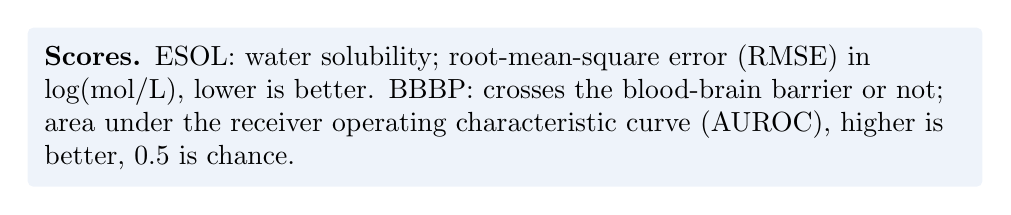
\begin{tikzpicture}
\node[fill=tint,rounded corners=2pt,inner sep=6pt,text width=\dimexpr\textwidth-12pt\relax,align=left]
{\textbf{Scores.} ESOL: water solubility; root-mean-square error (RMSE) in
log(mol/L), lower is better. BBBP: crosses the blood-brain barrier or not; area
under the receiver operating characteristic curve (AUROC), higher is better,
0.5 is chance.};
\end{tikzpicture}
\note{Left column is what the last slide of check-in 1 promised for today. A
stage is one step of the plan registered before the runs: C varies
the size of the corpus, D varies what is in it. The exposure check was promised
for the final and is done. Stage D has its own slide.}
\end{frame}

% =====================================================================
\begin{frame}{Stage C, all labels: a solubility gain from pretraining is first
detectable at 25,000 molecules, and none further after}
\begin{columns}[c,onlytextwidth]
\column{0.60\textwidth}
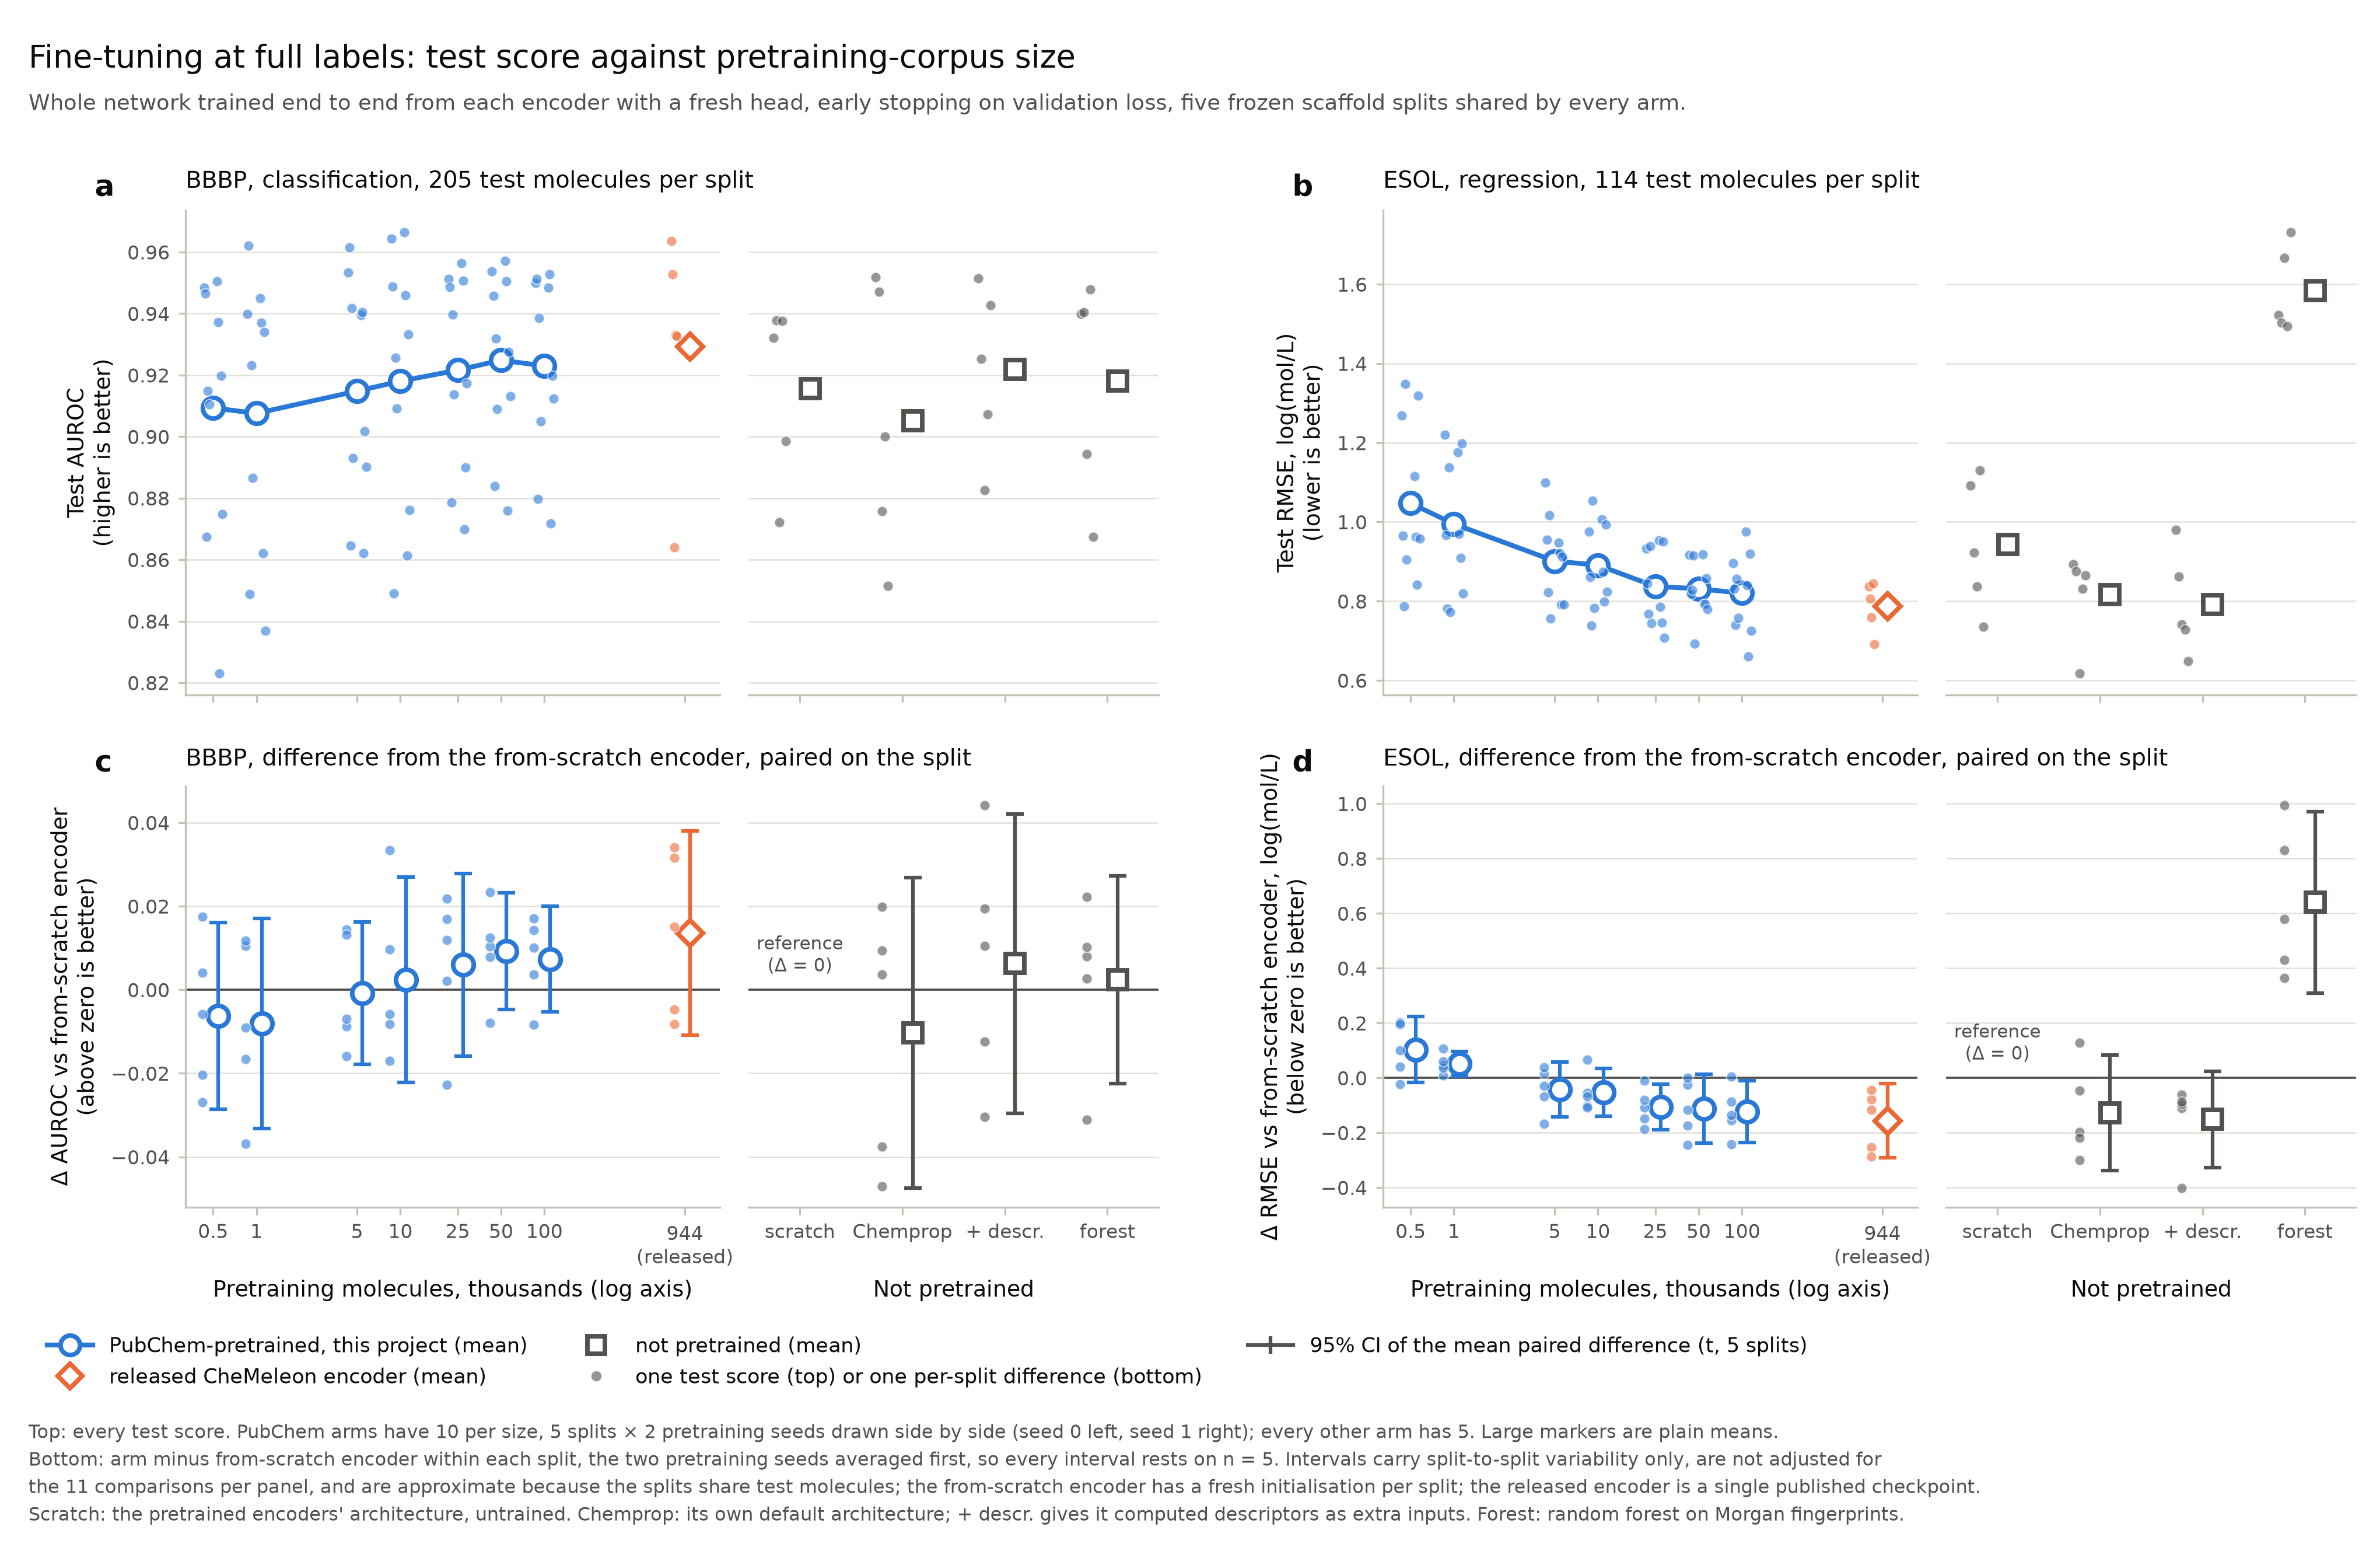
\includegraphics[width=\linewidth]{../figures/finetune_size_curve.png}
\column{0.37\textwidth}\raggedright
\textbf{Solubility} \muted{(ESOL, right)}\\[1mm]
Error falls as the corpus grows up to 25,000 molecules. Beyond that the means
keep falling slightly, but no further gain is detectable.\\[3mm]
\textbf{Blood-brain barrier} \muted{(BBBP, left)}\\[1mm]
No corpus size is separable from the untrained encoder.\\[3mm]
{\footnotesize\muted{All training labels. Bottom row: difference from the
untrained encoder on the same split; bars are 95\% intervals over five
splits.}\par}
\end{columns}
\note{Read the right-hand panels first. Horizontal axis: molecules in the
pretraining corpus, log scale, all drawn from PubChem. The orange diamond is
the encoder the CheMeleon authors released. The grey squares are models that
were never pretrained. Top row is the score, bottom row is the difference from
the same network left untrained. On the left no corpus size is separable from
the untrained encoder: say so and move on.}
\end{frame}

% =====================================================================
\begin{frame}{With all labels: no detectable gain below 25,000 molecules, and
none over Chemprop with descriptors at any size}
\begin{columns}[c,onlytextwidth]
\column{0.56\textwidth}
\begingroup\small\renewcommand{\arraystretch}{0.92}
\begin{tabular}{@{}L{36mm}r@{\hspace{5mm}}l@{}}
\toprule
\muted{Pretraining molecules} & \muted{RMSE} & \muted{Minus untrained}\\
\midrule
500 & 1.05 & +0.10 [\textminus 0.02, +0.22]\\
1,000 & 0.99 & \key{+0.05 [+0.01, +0.10]}\\
5,000 & 0.90 & \textminus 0.04 [\textminus 0.14, +0.06]\\
10,000 & 0.89 & \textminus 0.05 [\textminus 0.14, +0.04]\\
25,000 & 0.84 & \key{\textminus 0.11 [\textminus 0.19, \textminus 0.02]}\\
50,000 & 0.83 & \textminus 0.11 [\textminus 0.24, +0.01]\\
100,000 & 0.82 & \key{\textminus 0.12 [\textminus 0.24, \textminus 0.01]}\\
944,286, released & 0.79 & \key{\textminus 0.16 [\textminus 0.29, \textminus 0.02]}\\
\midrule
Untrained encoder & 0.94 & \muted{reference}\\
Chemprop & 0.82 & \textminus 0.13 [\textminus 0.34, +0.08]\\
Chemprop + descriptors & 0.79 & \textminus 0.15 [\textminus 0.33, +0.02]\\
\bottomrule
\end{tabular}\par\endgroup
\column{0.42\textwidth}\raggedright\small
\begin{itemize}
\setlength{\itemsep}{1.5mm}
\item Below 25,000 molecules: no detectable gain. At 1,000, slightly worse.
\item From 25,000: 0.11 to 0.16 better, with intervals barely clear of zero,
and not clear at 50,000.
\item \key{Chemprop + descriptors}, never pretrained: 0.79. Released minus
it: \textminus 0.005 [\textminus 0.13, +0.12]: not separable, which is not the
same as equal.
\end{itemize}
\vspace{1mm}
{\footnotesize\muted{Random forest on Morgan fingerprints: 1.58.}\par}
\end{columns}

\vspace{1mm}
{\footnotesize\muted{ESOL, all training labels. RMSE in log(mol/L), lower is
better: a negative difference is a gain. Brackets: 95\% interval over five
splits; bold: it excludes zero. Chemprop: a graph network trained from
scratch; + descriptors: with computed (Mordred) descriptors as inputs.
Released: the encoder published by the CheMeleon authors.}\par}
\note{The table is the right-hand panels of the previous slide. Bold means the
interval excludes zero, in either direction: at 1,000 molecules it excludes
zero on the wrong side. The last row is the uncomfortable one. The pretraining
task is predicting computed descriptors, and handing the same kind of
descriptors to a model that was never pretrained gives the same mean as the
released encoder, 0.79. Do not say ``matches'': its own interval against the
untrained encoder includes zero, and the interval on released minus Chemprop
with descriptors is as wide as the whole pretraining effect. No encoder of any
size shows a detectable gain over it. The random forest, 1.58, is far behind.}
\end{frame}

% =====================================================================
\begin{frame}{With few labels pretraining helps solubility more, but we
changed that recipe after seeing results}
\begin{columns}[c,onlytextwidth]
\column{0.345\textwidth}
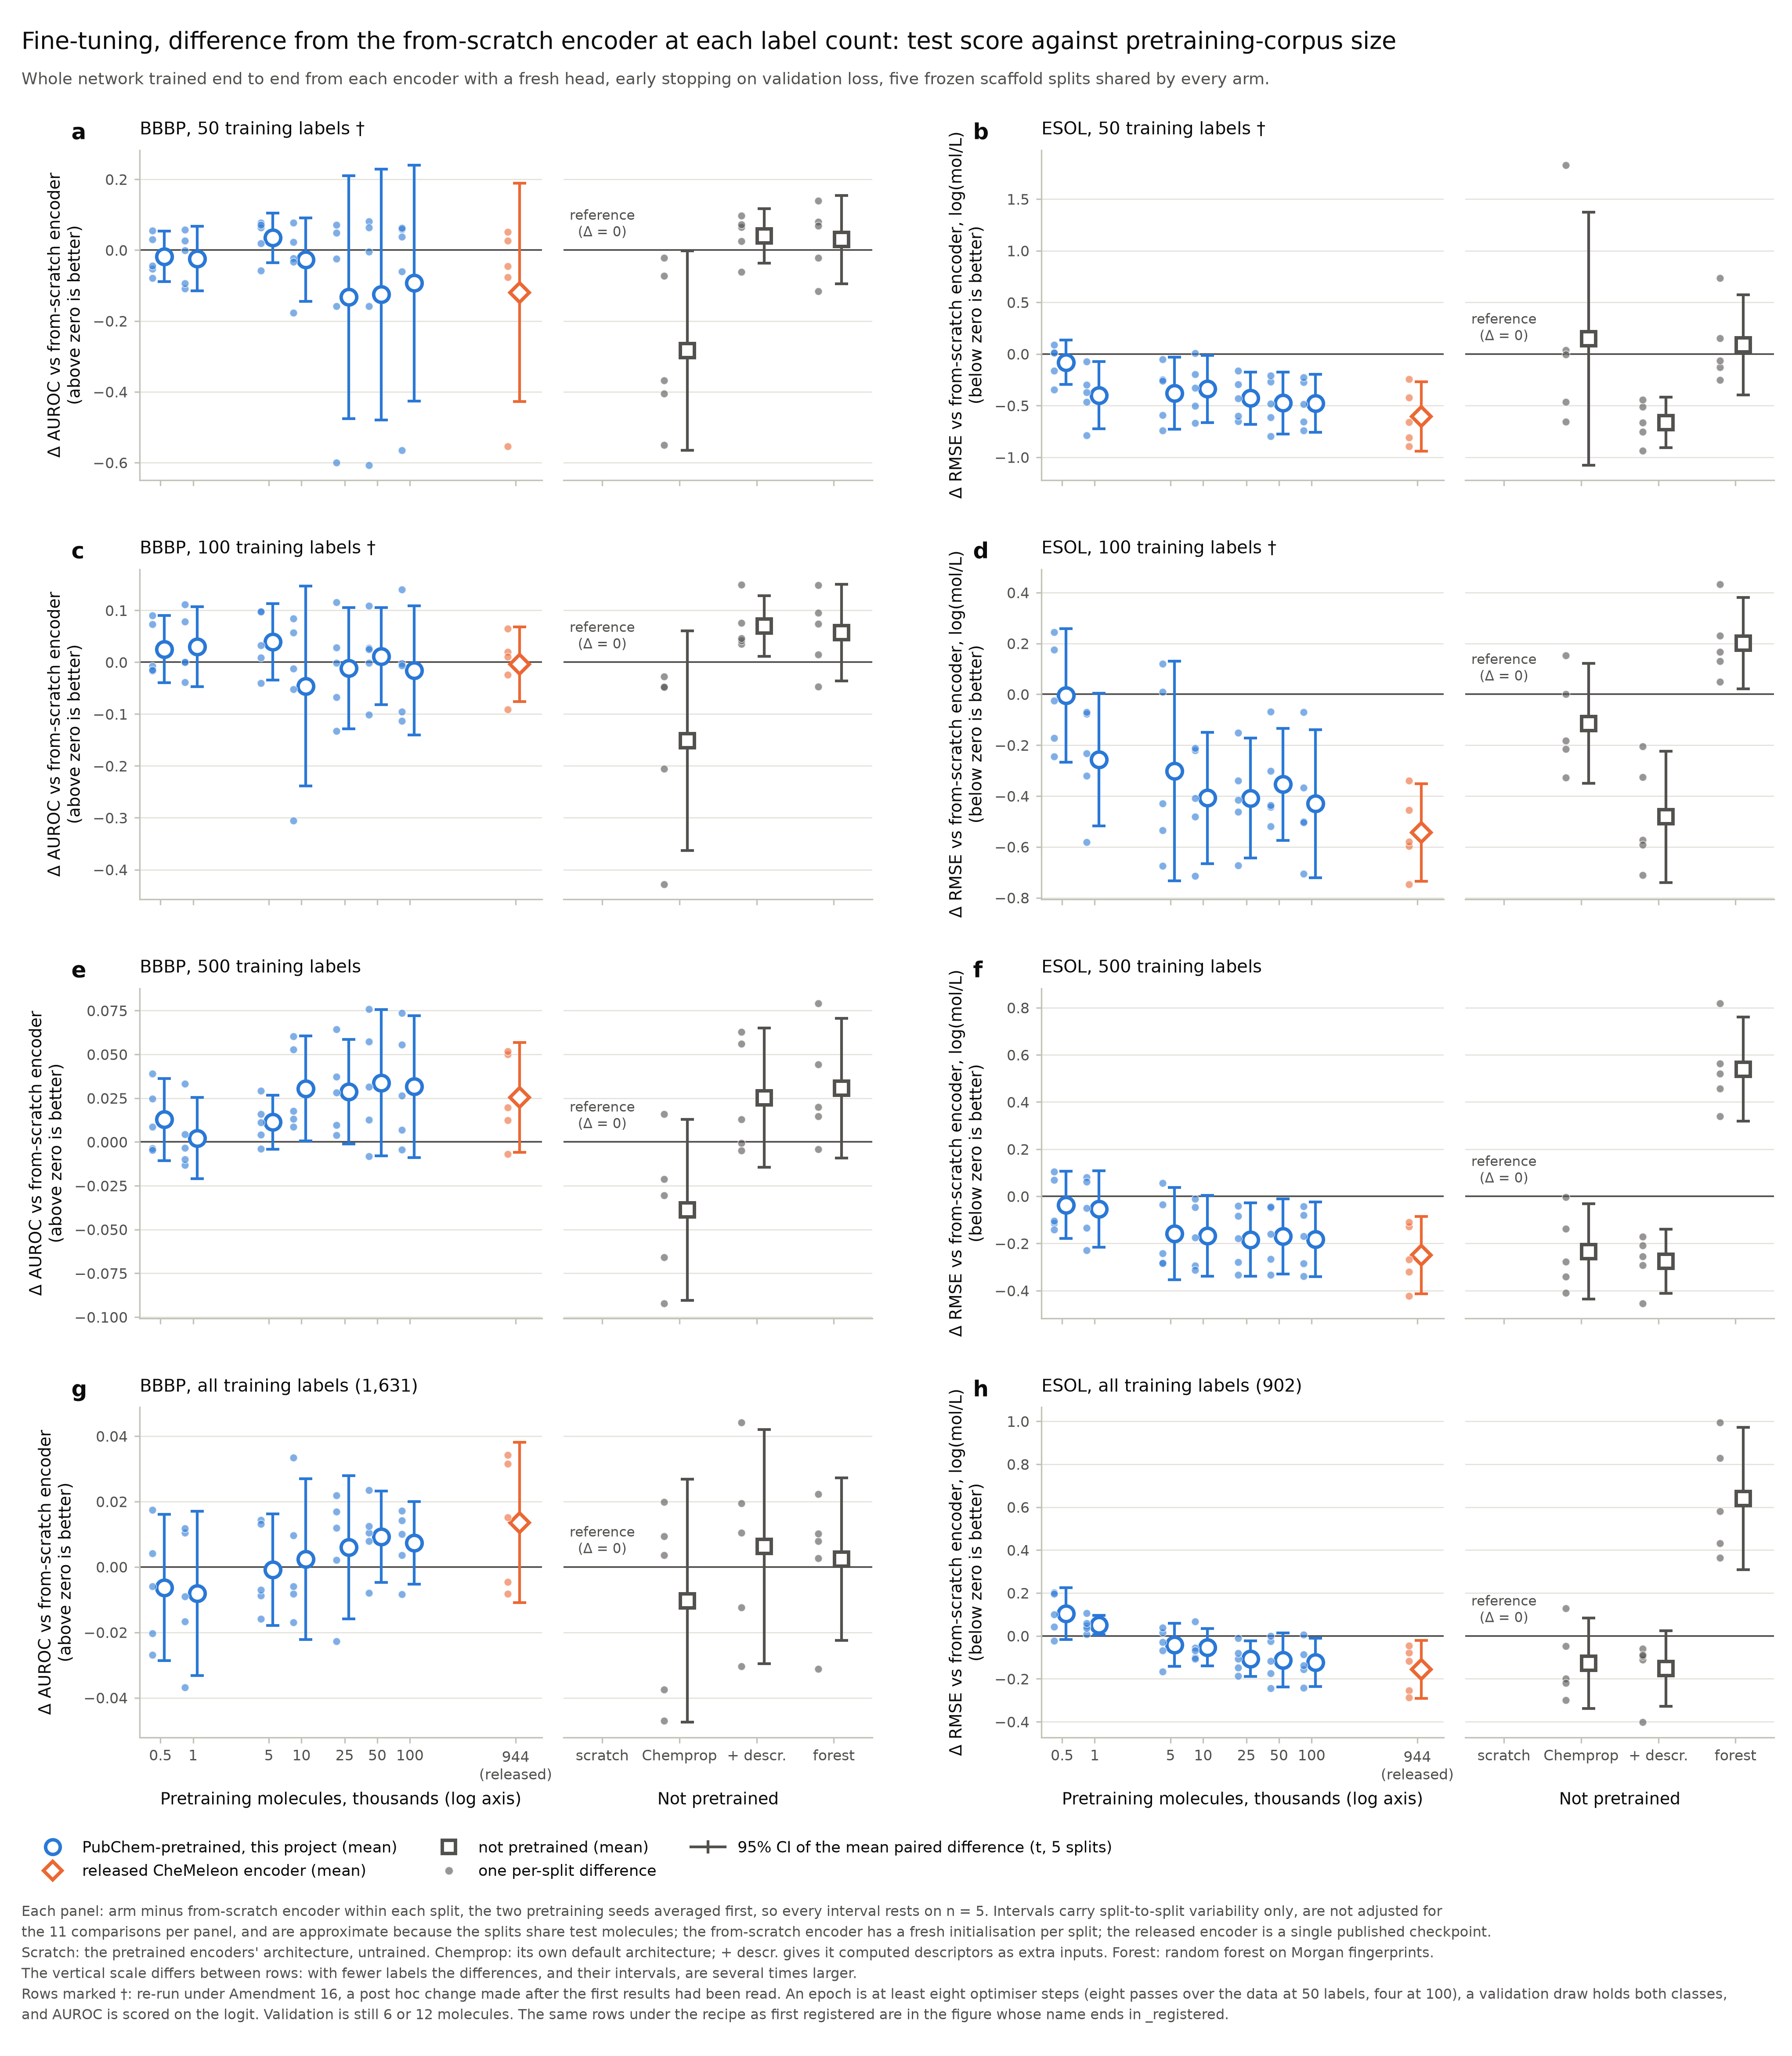
\includegraphics[height=56mm]{../figures/finetune_size_curve_by_labels.png}
\column{0.635\textwidth}\raggedright
\textbf{Amendment 16}, 13 November, for 50 and 100 labels
\begin{itemize}
\setlength{\itemsep}{1mm}
\item An epoch is at least eight optimiser steps. Before, it was one or two,
so training could stop after as few as ten or twenty steps.
\item A validation draw holds both classes; AUROC is scored on the logit, the
output before the sigmoid.
\end{itemize}
\key{Post hoc: written after the first scores were read.} Both versions are
kept.\\[1.5mm]
\begingroup\small
\begin{tabular}{@{}L{40mm}l@{}}
\toprule
\muted{Released, 50 labels} & \muted{ESOL RMSE, minus untrained}\\
\midrule
Recipe as registered & \textminus 0.72 [\textminus 0.90, \textminus 0.54]\\
Amended, shown here & \textminus 0.61 [\textminus 0.94, \textminus 0.27]\\
\bottomrule
\end{tabular}\par\endgroup
\vspace{1mm}
{\footnotesize\muted{On BBBP no gain from pretraining is detectable at 50 or
100 labels.}\par}
\end{columns}
\note{Rows of the figure, top to bottom: 50, 100, 500 and all training labels.
BBBP on the left, ESOL on the right. Every panel is a difference from the
untrained encoder. Only the top two rows were re-run. Be plain about the order
of events: the registered recipe counted in epochs, an epoch at 50 labels was
a single step, the runs were barely trained, and we saw that in the scores
before writing the fix. The rule has no tunable value, which is the defence.
The solubility gain is there under both recipes; its size is not settled.}
\end{frame}

% =====================================================================
\begin{frame}{Benchmark exposure is not visible in the scores: removing
benchmark molecules stays within seed-to-seed variation}
\begingroup\small % not a brace group: beamer would read it as a subtitle
\begin{tabular}{@{}L{56mm}L{38mm}L{40mm}@{}}
\toprule
\muted{100,000 PubChem molecules, all labels} & \muted{BBBP, AUROC, higher is
better} & \muted{ESOL, RMSE in log(mol/L), lower is better}\\
\midrule
Benchmark molecules kept & 0.925 & 0.816\\
Benchmark molecules removed & 0.925 & 0.799\\[2pt]
Removed minus kept & +0.001 [\textminus 0.006, +0.007] & \textminus 0.017 [\textminus 0.087, +0.052]\\
Second seed minus first, both kept & \textminus 0.004 [\textminus 0.016, +0.008] & +0.008 [\textminus 0.074, +0.089]\\
\bottomrule
\end{tabular}\par\endgroup

\vspace{4mm}
\begin{itemize}
\setlength{\itemsep}{2mm}
\item With every BBBP and ESOL molecule removed from the corpus, the change
sits inside the seed-to-seed interval on both tasks. At 50, 100 and 500 labels
its interval also includes zero.
\item \key{What this supports: ``not distinguishable from seed to seed'', not
``zero''.}
One encoder, on a fresh draw of the corpus.
\end{itemize}

\vspace{1mm}
{\footnotesize\muted{Brackets: 95\% interval over five splits, paired on the
split.}}
\note{This answers the obstacle slide of check-in 1: PubChem holds most of the
benchmark molecules. No label can leak, since pretraining never sees a
measurement; the worry was exposure to the structures. The last row is the
yardstick: the same recipe on another draw and another seed, which is a
difference that means nothing. The intervals on solubility are wide, so a small
effect could hide inside them.}
\end{frame}

% =====================================================================
\begin{frame}{The probe's odd solubility result was an artefact of
standardising near-dead dimensions; a cap fixes it}
\begin{columns}[c,onlytextwidth]
\column{0.48\textwidth}
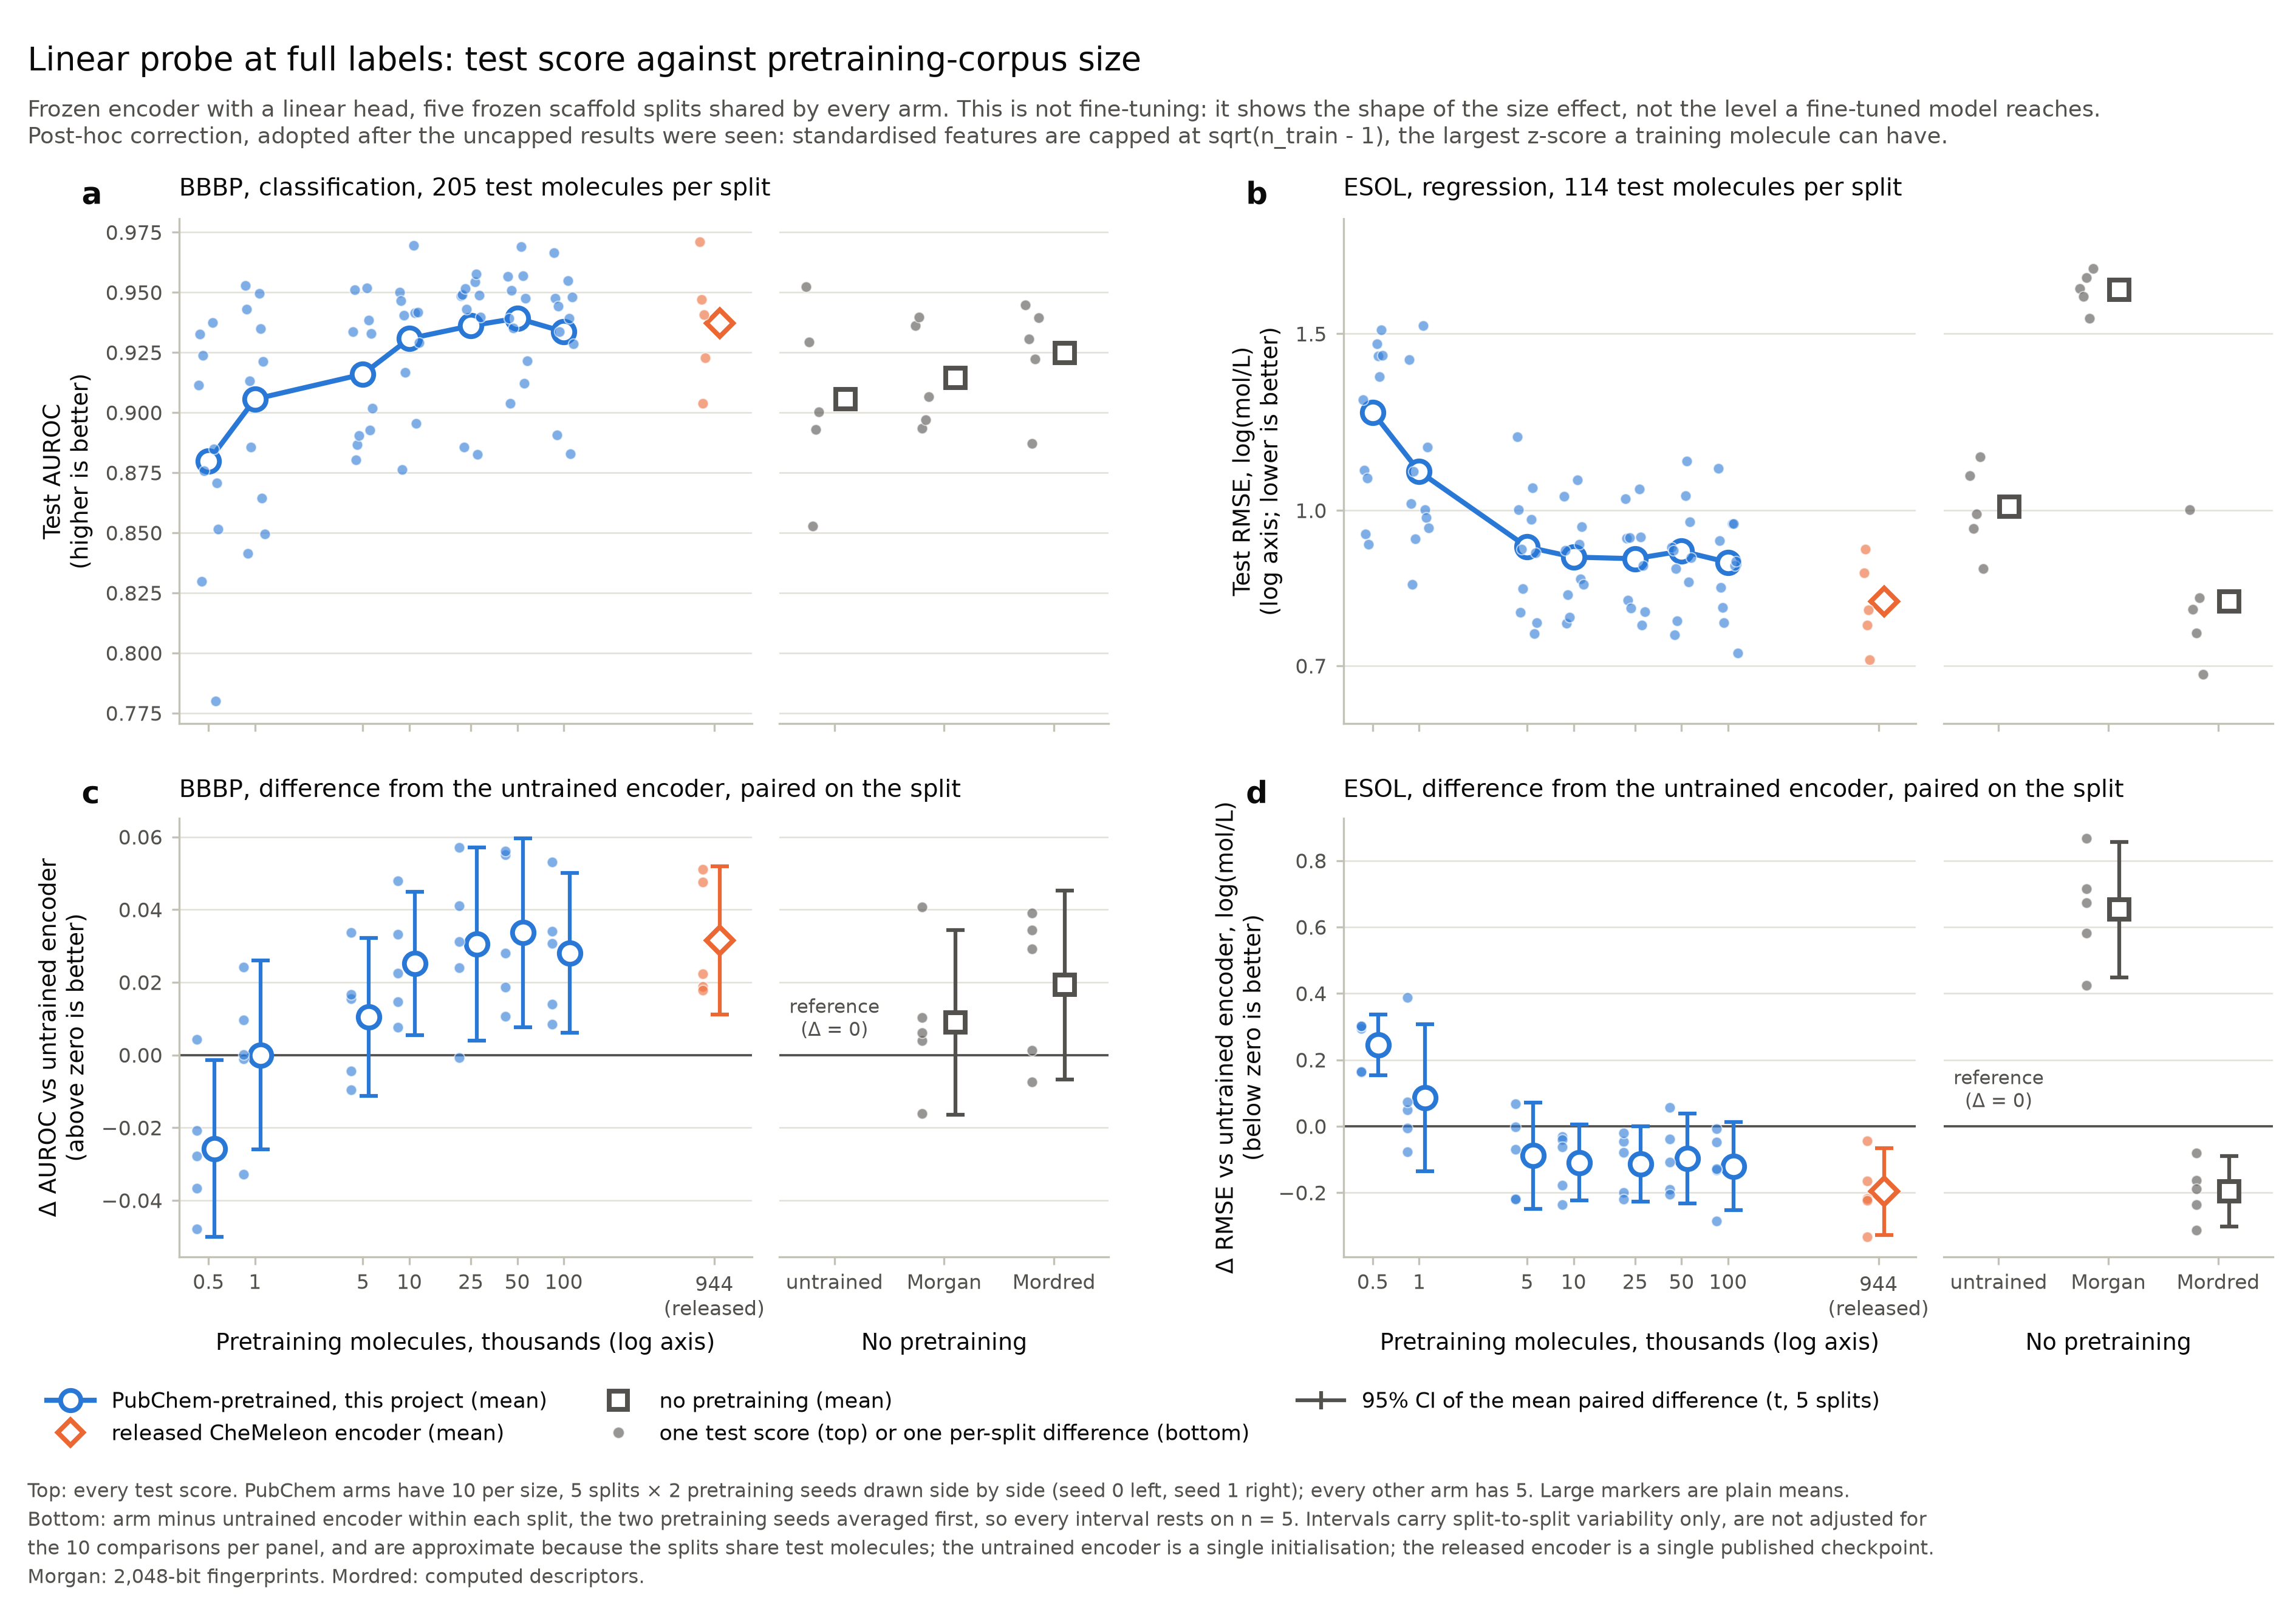
\includegraphics[width=\linewidth]{../figures/probe_full_labels_paired_clipped.png}
\column{0.49\textwidth}\raggedright
\textbf{Linear probe:} the encoder is frozen and only a linear layer is
trained on its output.\\[2.5mm]
\begingroup\small
\begin{tabular}{@{}l@{\hspace{3mm}}r@{\hspace{3mm}}l@{}}
\toprule
\muted{Released} & \muted{RMSE} & \muted{Minus untrained}\\
\midrule
No cap & 1.52 & +0.11 [\textminus 0.37, +0.59]\\
With cap & 0.81 & \key{\textminus 0.20 [\textminus 0.33, \textminus 0.07]}\\
\bottomrule
\end{tabular}\par\endgroup
\vspace{1mm}
\textbf{Cause:} a few output dimensions are almost constant, and dividing by
their tiny spread blows up test molecules.\\[1.5mm]
\textbf{Fix:} cap the standardised values. \key{Post~hoc.}
\end{columns}

\vspace{2mm}
{\footnotesize\muted{ESOL, all labels, RMSE in log(mol/L), lower is better;
95\% interval over five splits. The untrained encoder moved too, from 1.41 to
1.01. Figure: with the cap.}\par}
\note{The probe is the cheap companion to fine-tuning: it asks what is already
in the encoder's output. Without the cap the released encoder, the best one
after fine-tuning, looked worse than an untrained network on solubility, and
every interval on solubility was wide. That was the clue. The cap was adopted
after seeing those numbers and the figure says so in its subtitle. Both tables
are kept.}
\end{frame}

% =====================================================================
%% STAGE-D-FRAME-BEGIN
\begin{frame}{Stage D: at 25,000 molecules, five splits do not separate the
three corpora}
\begin{columns}[c,onlytextwidth]
\column{0.59\textwidth}
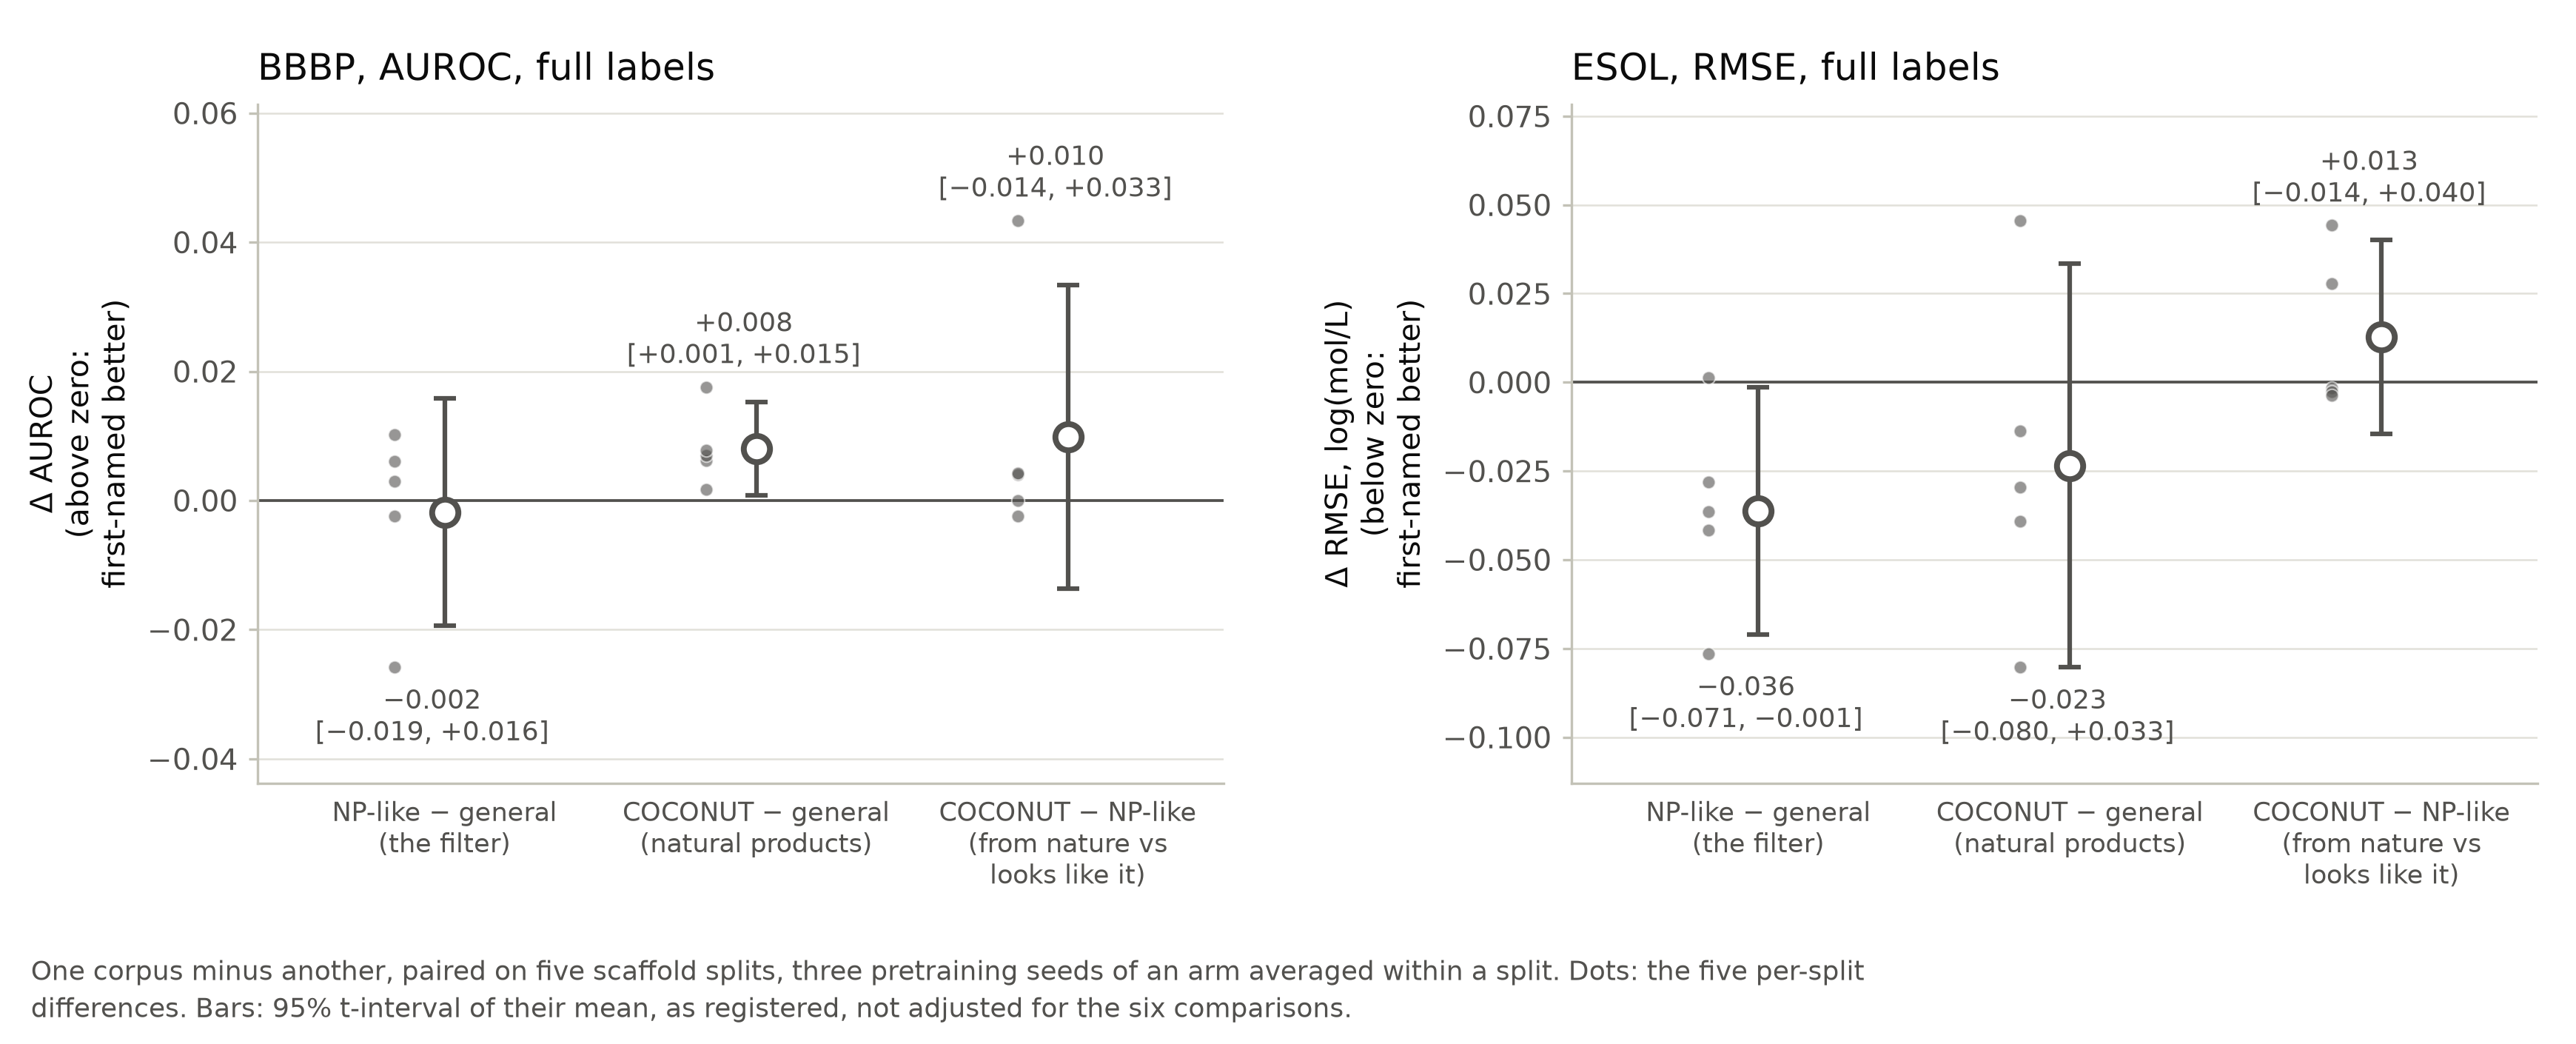
\includegraphics[width=\linewidth]{../figures/stage_d_composition_slide.png}
\column{0.38\textwidth}\raggedright\small
\textbf{Largest gaps:} 0.036 RMSE on solubility, 0.010 AUROC on blood-brain
barrier.\\[3mm]
\textbf{Two of six intervals exclude zero,} both against ZINC general, both
by a hair. \key{Neither survives adjustment for six comparisons}
\muted{(adjusted $p$ = 0.22 and 0.27)}.\\[3mm]
\textbf{Not evidence of no effect:} the intervals leave room for up to 0.08
RMSE and 0.03 AUROC either way.
\end{columns}

\vspace{1mm}
{\footnotesize\muted{All training labels; the comparison registered in
Amendment 17. ZINC NP-like: the most natural-product-like tenth of ZINC
general. COCONUT: natural products.}}
\note{Each mark is one corpus minus another on the same five splits, so the
first-named corpus is better above zero on the left panel and below zero on
the right. The two intervals that clear zero are COCONUT over ZINC general on
blood-brain barrier, by 0.008 AUROC, and ZINC NP-like over ZINC general on
solubility, by 0.036 RMSE. Taken six at a time neither holds. Say plainly that
this is a null with wide intervals, not a demonstration that composition does
not matter. All 360 runs are in: three corpora, three seeds, two tasks, five
splits, four label budgets.}
\end{frame}

% =====================================================================
\begin{frame}{With few labels all three corpora help solubility; with all
labels none is separable from the untrained encoder}
\begingroup\small
\begin{tabular}{@{}L{27mm}l@{\hspace{5mm}}l@{\hspace{5mm}}l@{}}
\toprule
\muted{Training labels} & \muted{ZINC general} & \muted{ZINC NP-like} & \muted{COCONUT}\\
\midrule
50 labels & \key{\textminus 0.35 [\textminus 0.62, \textminus 0.09]} & \key{\textminus 0.41 [\textminus 0.69, \textminus 0.14]} & \key{\textminus 0.43 [\textminus 0.72, \textminus 0.13]}\\
100 labels & \key{\textminus 0.32 [\textminus 0.54, \textminus 0.10]} & \key{\textminus 0.36 [\textminus 0.56, \textminus 0.16]} & \key{\textminus 0.39 [\textminus 0.63, \textminus 0.16]}\\
500 labels & \textminus 0.13 [\textminus 0.29, +0.04] & \textminus 0.13 [\textminus 0.28, +0.01] & \key{\textminus 0.15 [\textminus 0.30, \textminus 0.002]}\\
All 902 labels & \textminus 0.04 [\textminus 0.16, +0.07] & \textminus 0.08 [\textminus 0.18, +0.02] & \textminus 0.07 [\textminus 0.16, +0.03]\\
\bottomrule
\end{tabular}\par\endgroup

\vspace{2mm}
\begingroup\small
\begin{itemize}
\setlength{\itemsep}{1.5mm}
\item At 50 and 100 labels every corpus gains 0.32 to 0.43, in five of five
splits; with all labels 0.04 to 0.08, and no interval excludes zero.
\item \key{ZINC general has the worst mean at all four budgets}, by 0.01 to
0.07: one pattern on the same encoders and splits, not four results.
\item Blood-brain barrier: no corpus is separable from the untrained encoder
at any budget \muted{(0 of 12 intervals exclude zero)}.
\end{itemize}
\endgroup

\vspace{1mm}
{\footnotesize\muted{ESOL, RMSE of each encoder minus the untrained one, in
log(mol/L): negative is a gain. Brackets: 95\% interval over five splits;
bold: it excludes zero.}}
\note{The registered comparison sits at full labels, which is where
pretraining itself is hardest to see at this corpus size, so there is little
room there for composition to show. Where pretraining clearly helps, with 50
or 100 labels, the corpus-to-corpus intervals are wide, plus or minus 0.07 to
0.16. The 50 and 100 label rows rest on 6 or 12 validation molecules. ZINC
NP-like's three draws share half their molecules, because its pool is only
49,997 molecules, so that arm is closer to one corpus trained three times.}
\end{frame}
%% STAGE-D-FRAME-END

% =====================================================================
\begin{frame}{What limits these results: five splits, two tasks, unadjusted
intervals and two unsigned amendments}
\begin{itemize}
\setlength{\itemsep}{2mm}
\item \textbf{Five scaffold splits.} Every interval is a 95\% t-interval on
five paired differences.
\item \textbf{Two tasks, one of them nearly silent.} After fine-tuning with
all labels, BBBP separates no corpus size from the untrained encoder; over all
four label budgets one interval of 32 excludes zero, by 0.0005. The evidence
is ESOL alone.
\item \textbf{Intervals are not adjusted} for the number of comparisons.
Several exclude zero only just; none should be read alone.
\item \textbf{Two fixes came after the results.} Amendment 16 for 50 and 100
labels, and the cap in the probe. Both versions of each are kept.
\item \textbf{Low labels are still fragile.} 108 of the 360 repeated runs
still restore their first checkpoint.
\item \textbf{Amendments 16 and 17 are not yet signed} by the second author,
L\'eonard.
\end{itemize}
\note{Do not rush this slide. The honest summary: one task shows an effect, on
five splits, with intervals that were not corrected for how many we looked at.
Amendment 17 fixes Stage D: three corpora, 25,000 molecules, three seeds,
benchmark molecules excluded. It was written before any Stage D corpus was
drawn but after Stage C was read, and by one of us.}
\end{frame}

% =====================================================================
\begin{frame}{Next: find where the gain lives, write up by 1 December, and
decide on a natural-product task}
\begin{columns}[t,onlytextwidth]
\column{0.37\textwidth}\raggedright
{\color{accent}\rule{\linewidth}{1.2mm}}\\[1.5mm]
\textbf{Stage E: where does any gain live?}\\[2mm]
Group the test molecules by similarity to the pretraining corpus\\[1.5mm]
Measure the gain in each group\\[1.5mm]
No new training
\column{0.27\textwidth}\raggedright
{\color{hair}\rule{\linewidth}{1.2mm}}\\[1.5mm]
\textbf{Write-up, due 1 December}\\[2mm]
Results frozen on 29 November\\[1.5mm]
Both amendments signed by both authors
\column{0.30\textwidth}\raggedright
{\color{hair}\rule{\linewidth}{1.2mm}}\\[1.5mm]
\textbf{Open decision}\\[2mm]
Add a task nearer natural-product chemistry?\\[1.5mm]
If so: by amendment, and for all nine Stage D encoders at once
\end{columns}

\vspace{2mm}
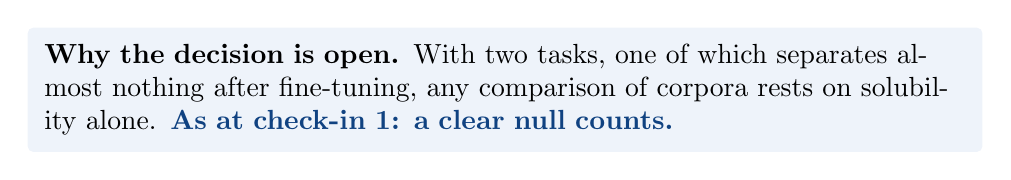
\begin{tikzpicture}
\node[fill=tint,rounded corners=2pt,inner sep=6pt,text width=\dimexpr\textwidth-12pt\relax,align=left]
{\textbf{Why the decision is open.} With two tasks, one of which separates
almost nothing after fine-tuning, any comparison of corpora rests on
solubility alone. \key{As at check-in 1: a clear null counts.}};
\end{tikzpicture}
\note{Stage E is the last item promised for the final at check-in 1: gain
against similarity to the corpus. It needs no new training, only the
predictions already on disk. The open decision is the one we would most like
advice on. Close on the title: same model, same training, different
molecules.}
\end{frame}

\end{document}
